\section{Ungesteuerter Gleichrichter}
\subsection{M1U}
\vspace{-0.5cm}
\begin{minipage}{0.4\linewidth}
    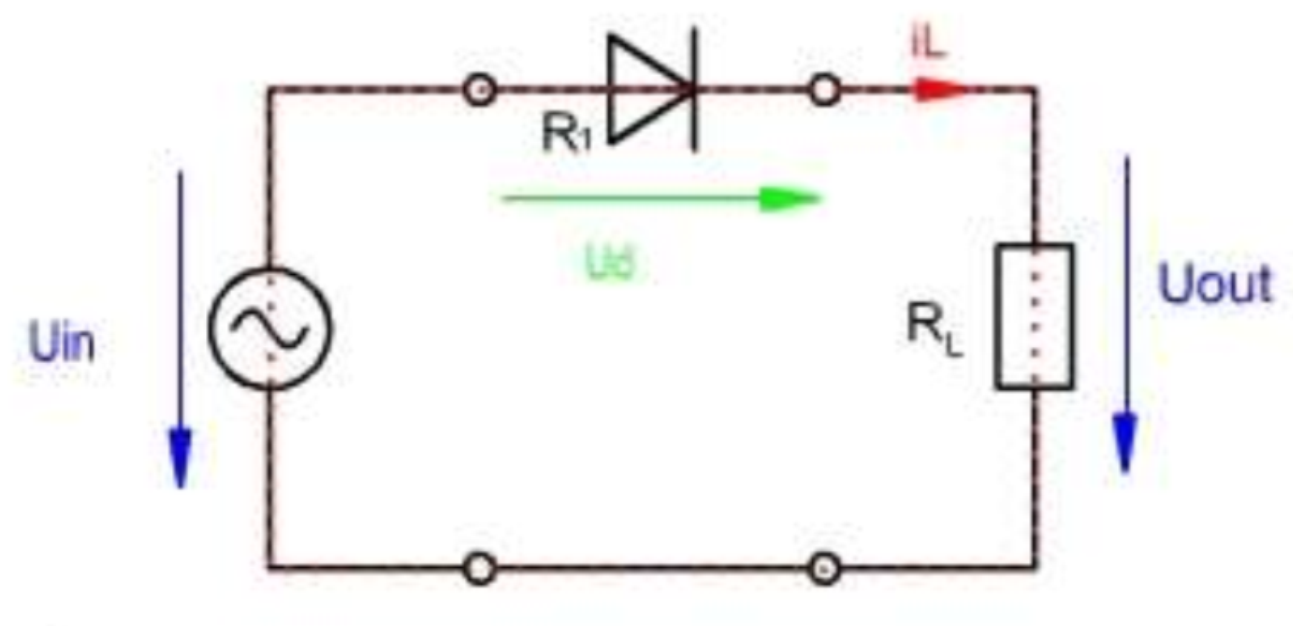
\includegraphics[width=\linewidth]{images/PrakUGM1}
\end{minipage}
\begin{minipage}{0.3\linewidth}
    \centering
   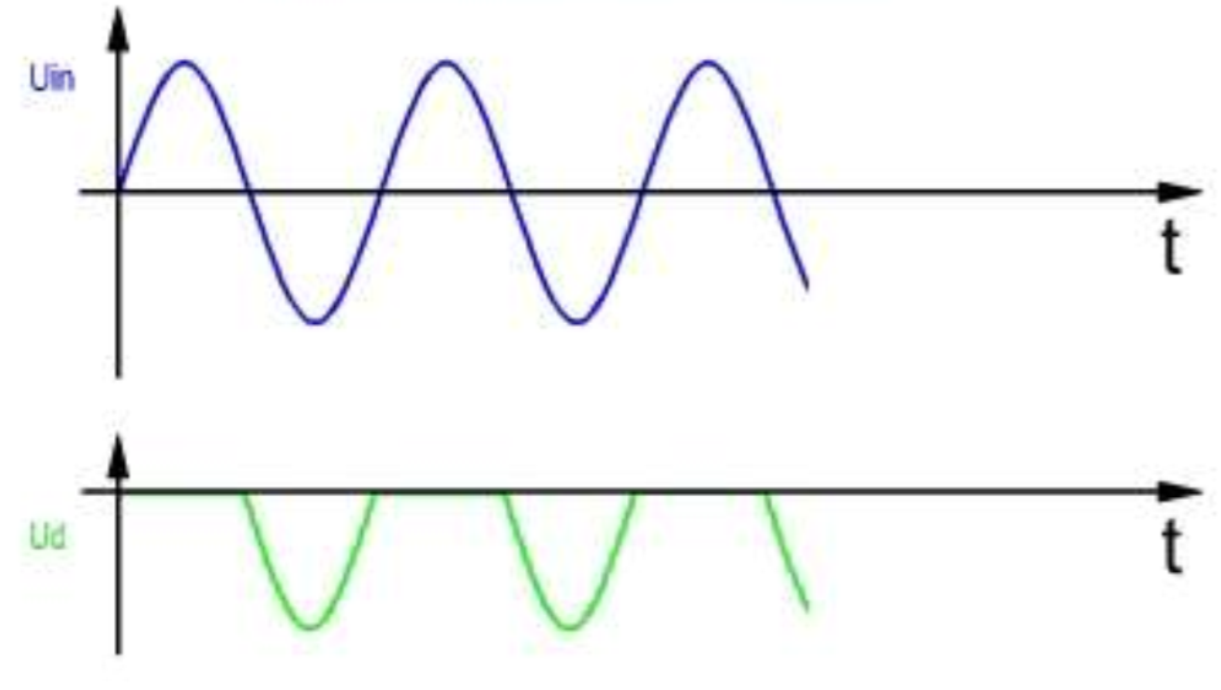
\includegraphics[width=0.7\linewidth]{images/PrakUGM1Kl1}
   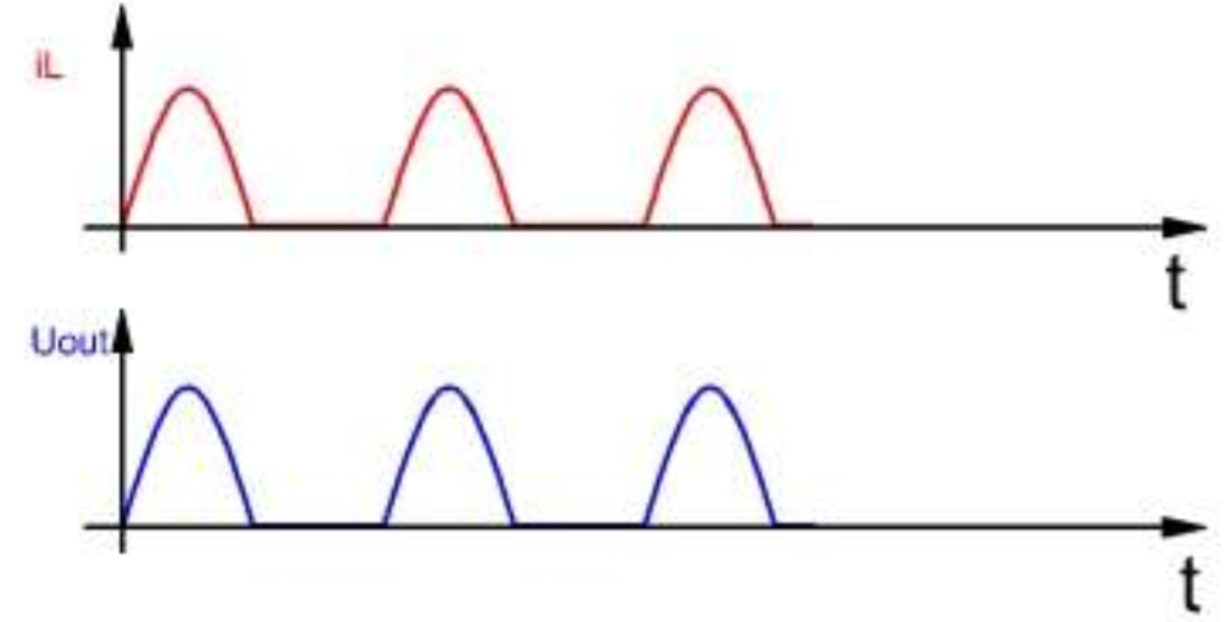
\includegraphics[width=0.7\linewidth]{images/PrakUGM1Kl2}
\end{minipage}
\begin{minipage}{0.3\linewidth}
    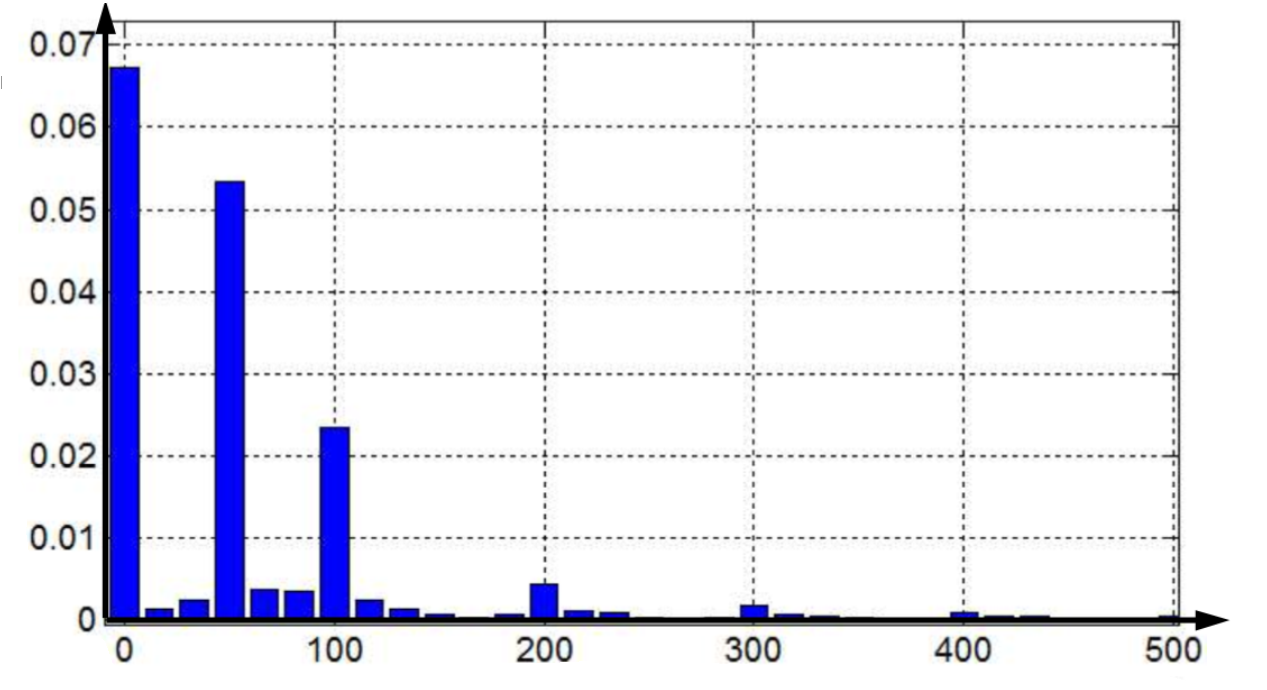
\includegraphics[width=\linewidth]{images/UGM1OW} 
\end{minipage}
\newline

%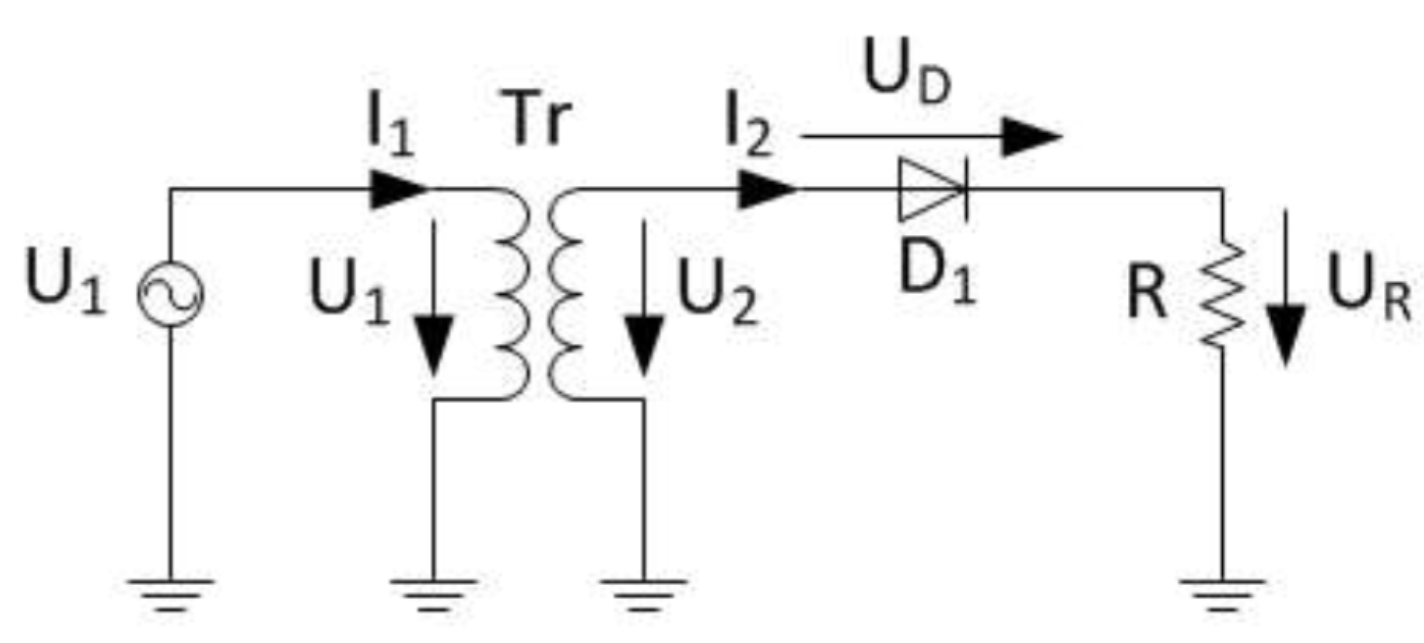
\includegraphics[width=0.4\linewidth]{images/UGRM1U}
%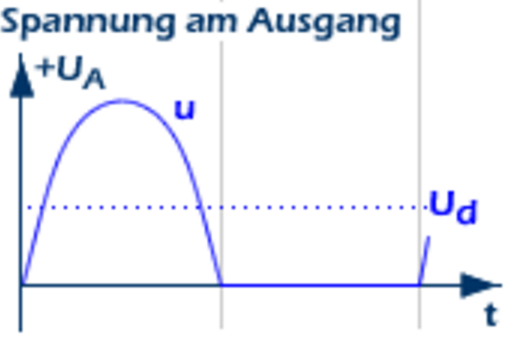
\includegraphics[width=0.2\linewidth]{images/UGRM1US} \newline
Die Diode wird als Ideal betrachtet $ \rightarrow $ keine Schwellenspannung oder Innenwiderstand
\begin{longtable}{| p{.3\textwidth} | p{.40\textwidth} | p{.25\textwidth} |} %TODO Formeln einfügen bzw anpassen
    \hline
    \textbf{Grundgleichungen}&
    \[ U_2 = U_D + U_R \]
    \[ U_R = I_2 \cdot R\]
    \[ \bar{U}_{OUT} = \dfrac{\hat{U}}{\pi}\]&
    \textbf{Durchlassrichtung}\newline
    $ 0 < \omega t < \pi $\newline
    $U_2 = U_R \qquad U_D = 0$\newline

    \textbf{Sperrichtung}\newline
    $ \pi < \omega t < 2\pi $\newline
    $ U_2=U_D \qquad U_R = 0 $\newline
    \\
    \hline
    
    \textbf{Wirkleistung der Last R}&
    \[ P=\frac{1}{2\pi} \int_{0}^{2\pi} p(\alpha) d\alpha = \dfrac{U_{R\;RMS}^2}{R} \]&
    \\ \hline
\end{longtable}

%
%Leistung = Momentanleistung des Sormes x momentanleistung der Spannung\\
%Leistung = Leistung bei trafoseite messen 1harm des stroms phasenverschiebung -> u i cos(phi) fourierreihen..
%Leistung = Irav* U1harm  
\textbf{Oberwellen}\newline
\vspace{-1cm}
\begin{multicols}{3}
    \textbf{ \qquad R}\newline   
    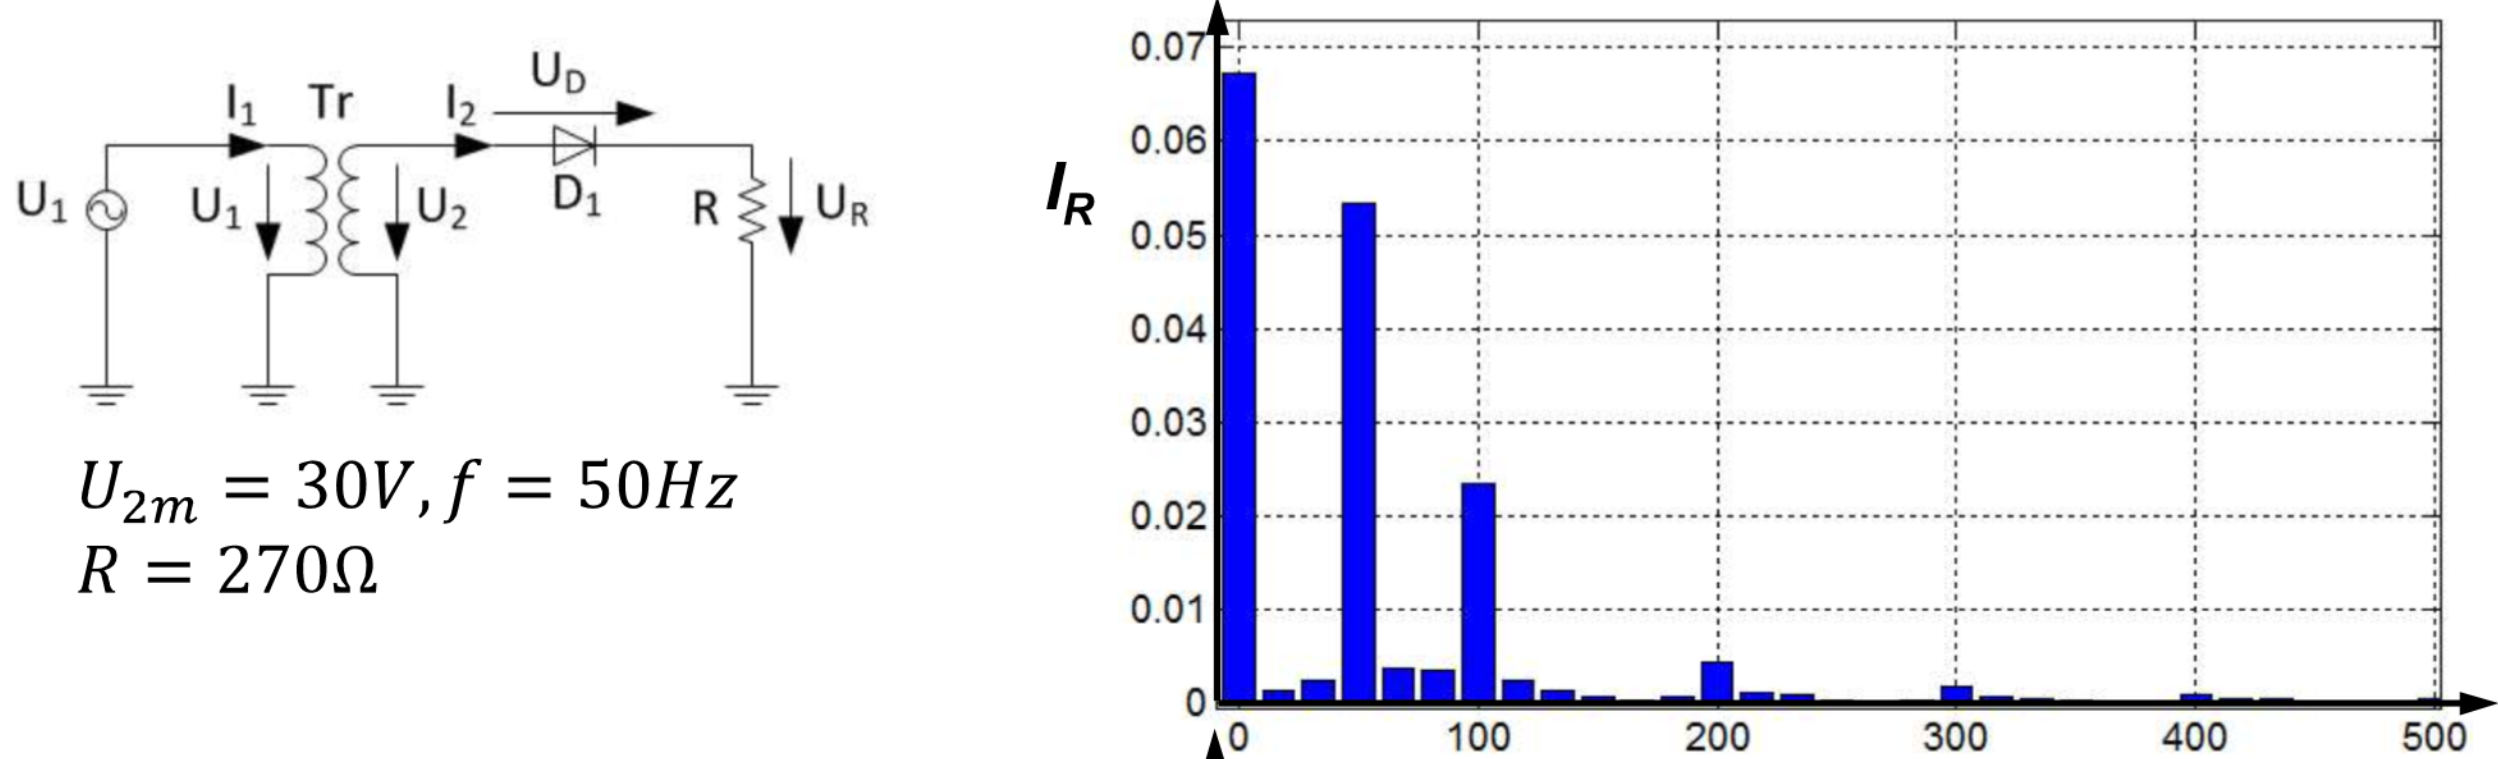
\includegraphics[width=\linewidth]{images/M1UR}   
    \textbf{\null \qquad R + L}\newline
    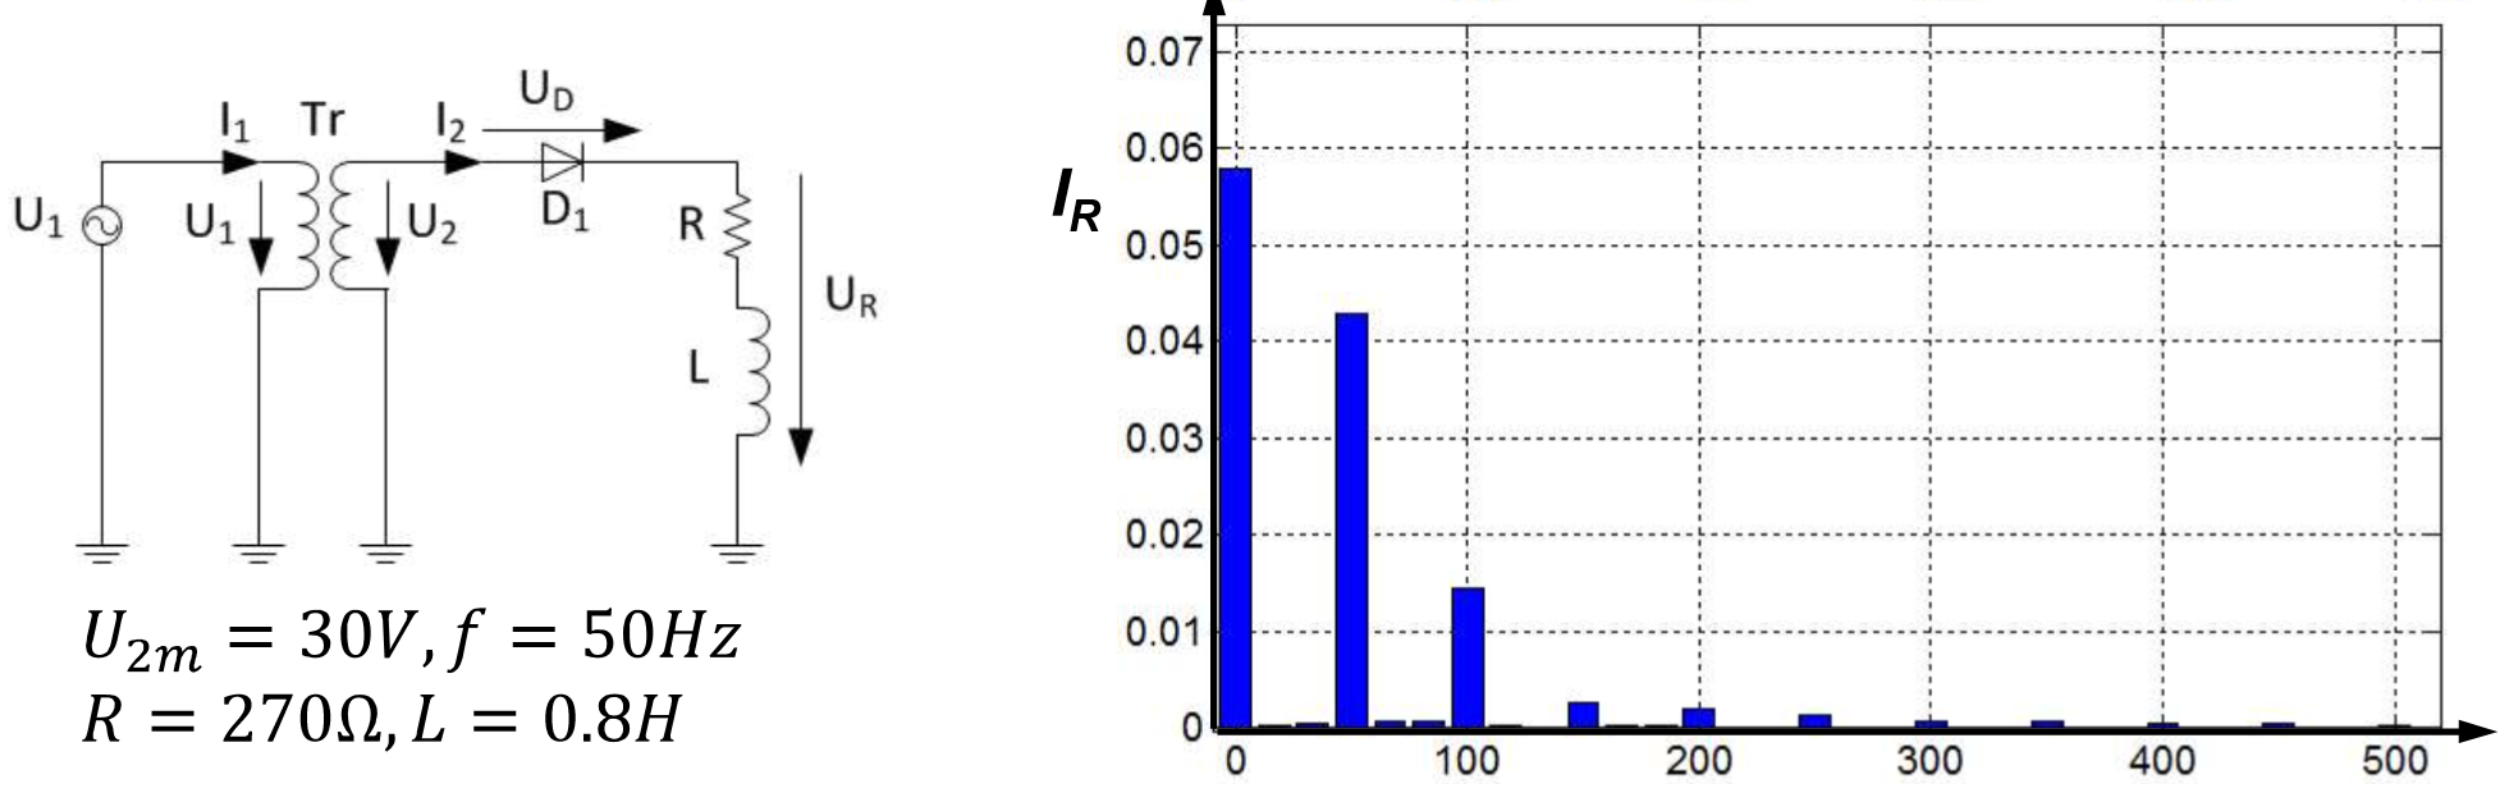
\includegraphics[width=\linewidth]{images/M1URL}
    \textbf{ \qquad R + L+ freilaufDiode}\newline
    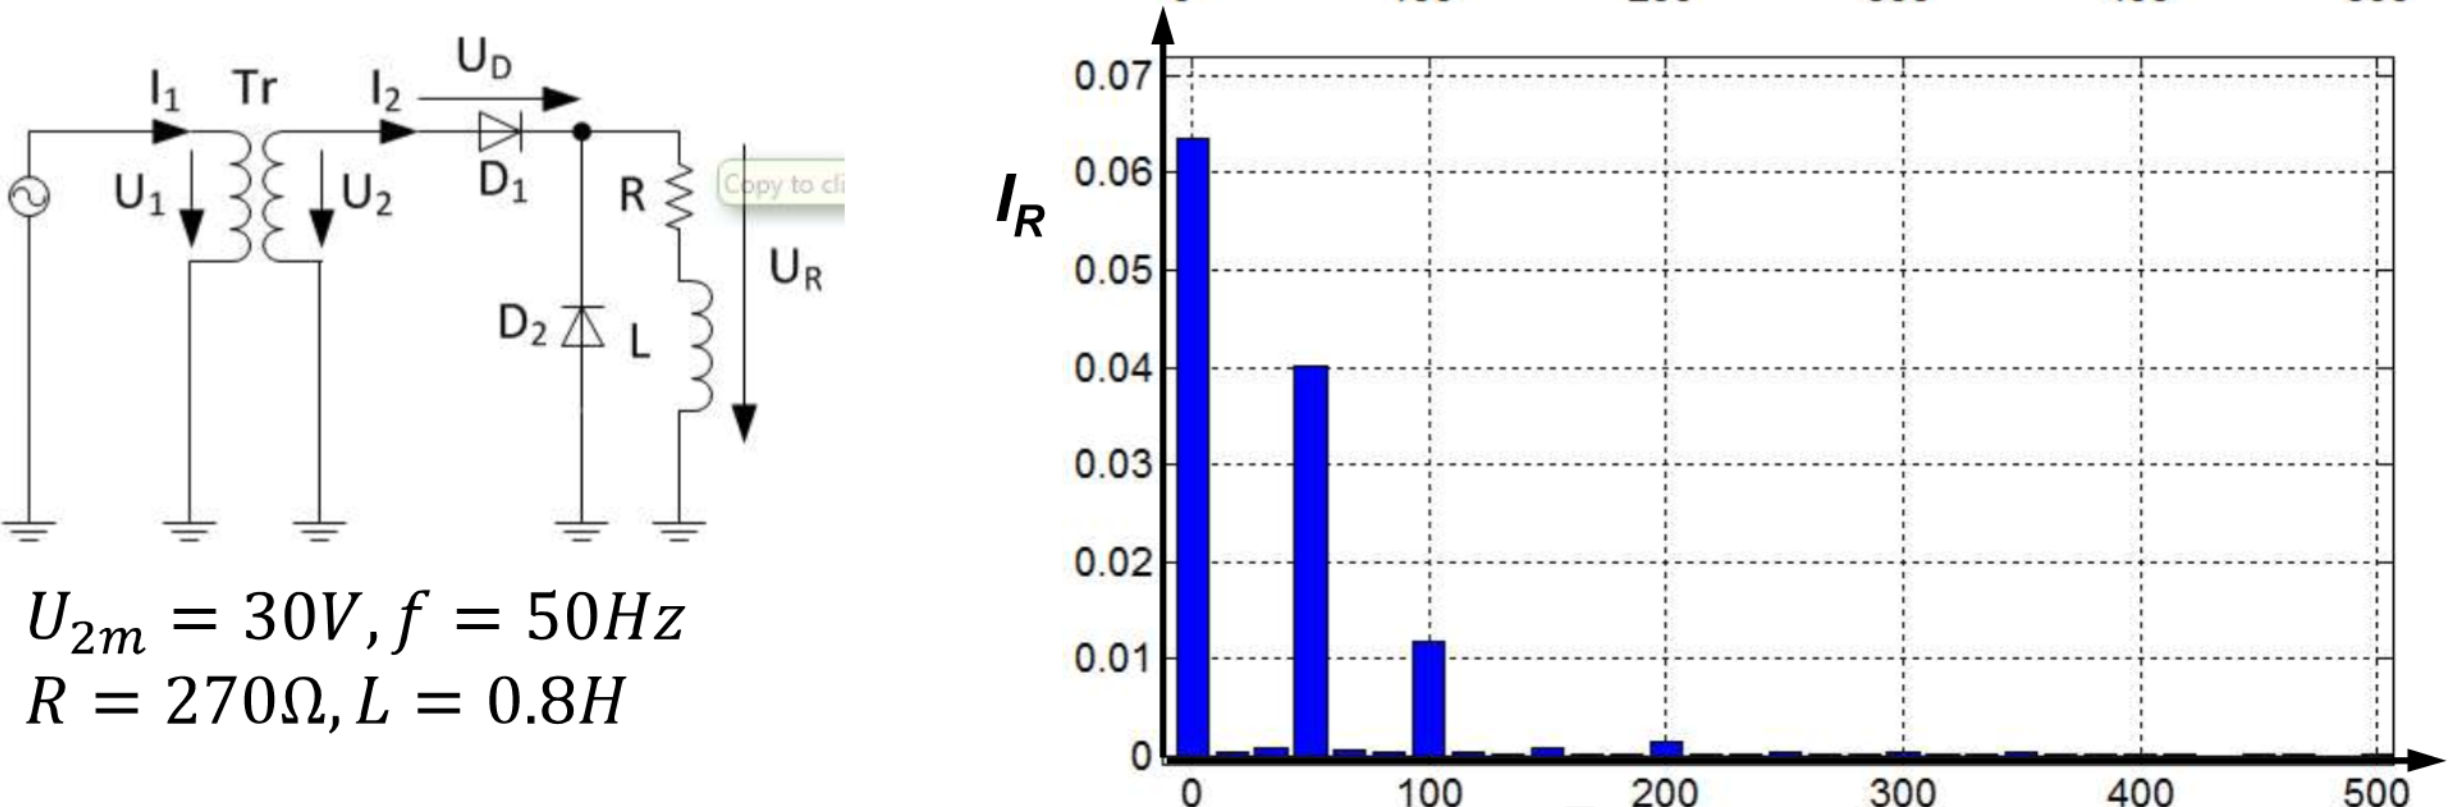
\includegraphics[width=\linewidth]{images/M1URLD}
\end{multicols}
\subsubsection{Rechnungsbsp.}
\textbf{Übung 2 - Gleichrichter M1U}\newline
\renewcommand{\arraystretch}{2}
\begin{tabular}{ p{.3\textwidth}  p{.40\textwidth}  p{.25\textwidth}}
    Ausgangslage:&
    $ U_2= U_{2m}\cdot sin(2\cdot \pi\cdot f\cdot t)$&
    \\
    Mittelwert Spannung: &
    $ U_{R \; AV}= \frac{1}{2 \pi} \int\limits_{0}^{\pi} U_{2m}\cdot sin(\alpha)\cdot\diff\alpha=\frac{U_{2m}}{\pi} $ &
    $ \alpha=\omega t $
    \\
    
    Effektivwert Spannung:   &
    $ U_{R \; RMS}= \sqrt{\frac{1}{2 \pi}\int\limits_{0}^{\pi} U_{2m}^2\cdot sin(\alpha)^2\cdot\diff\alpha} = \frac{U_{2m}}{2} $ &
    \\ 
    
    Mittelwert Strom: &
    $ I_{R \; AV}=\frac{U_{R \; AV}}{R_L}= \frac{1}{\pi}\frac{U_{2m}}{R}= \frac{1}{\pi} I_{2m} $ &
    \\
    
    Effektivwert Strom: &
    $ I_{R \; RMS}=\frac{U_{R \; RMS}}{R}= \frac{U_{2m}}{2\cdot R}= \frac{I_{2m}}{2} $ &
    \\
    
    Wirkleistung R: &
    $ P= \frac{1}{2\pi}\int\limits_{0}^{\pi}\frac{u_R^2(\alpha)}{R}\cdot \diff \alpha = \frac{U_{R \; RMS}^2}{R}=\frac{1}{R}\frac{U_{2m}^2}{4} $
\end{tabular}
\renewcommand{\arraystretch}{1}

%===================================================================
\clearpage

\subsubsection{B2U}
\begin{minipage}{0.4\textwidth}
    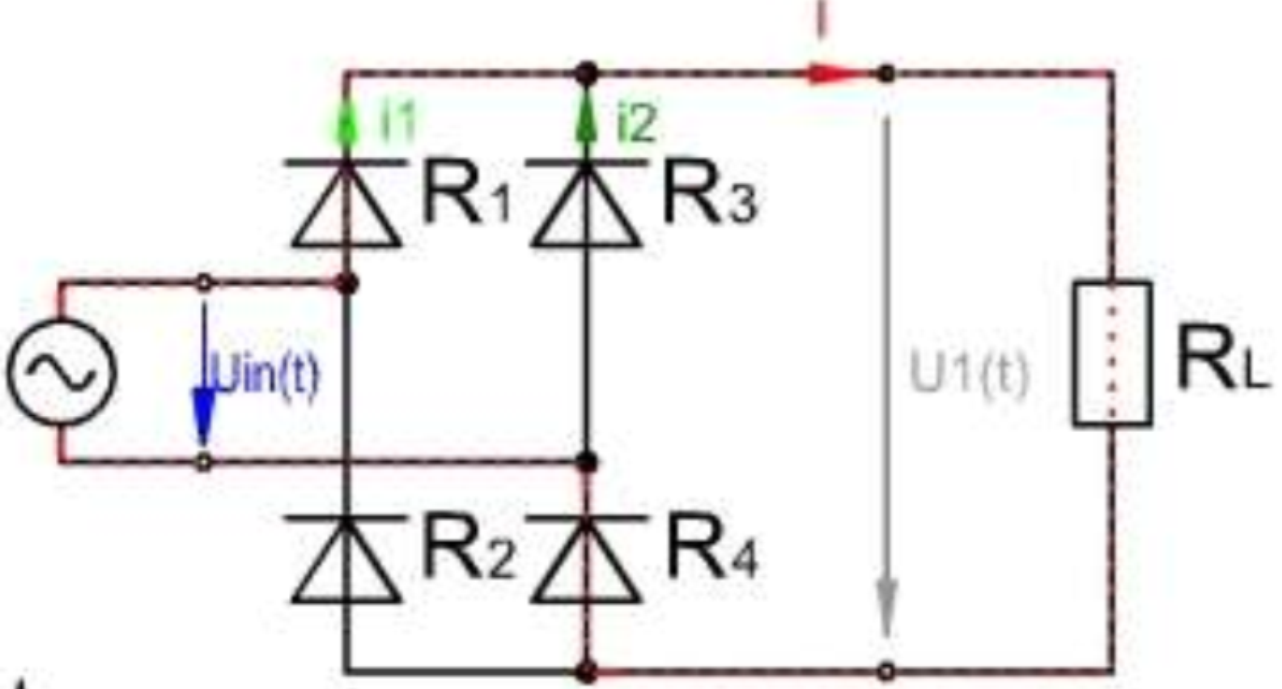
\includegraphics[width=\linewidth]{images/PrakUGB2}
\end{minipage}
\begin{minipage}{0.25\linewidth}
    \centering
    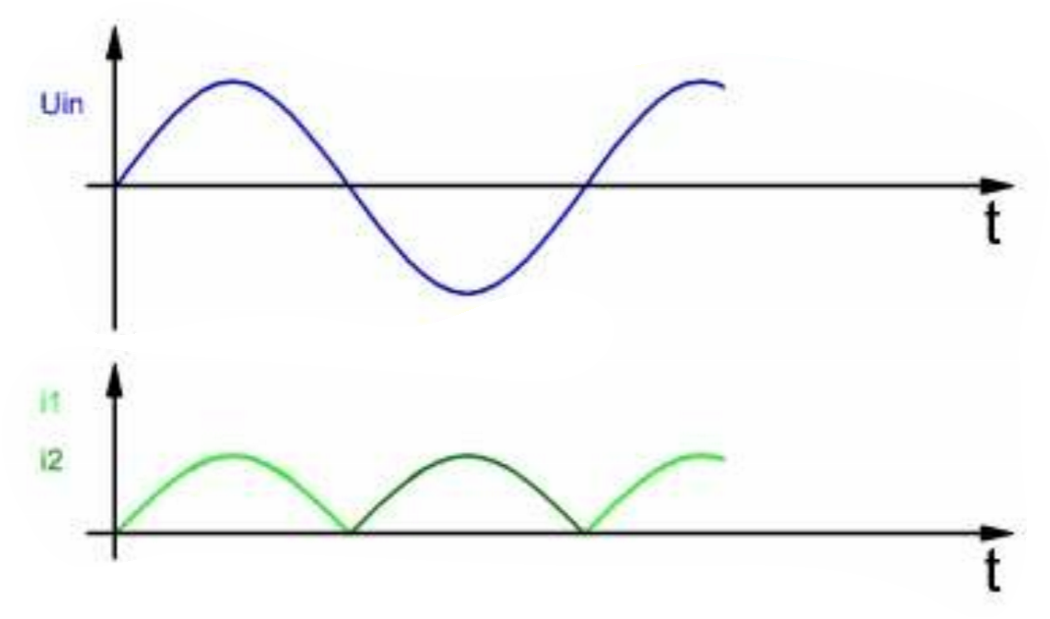
\includegraphics[width=0.9\linewidth]{images/PrakUGB2Kl1}
    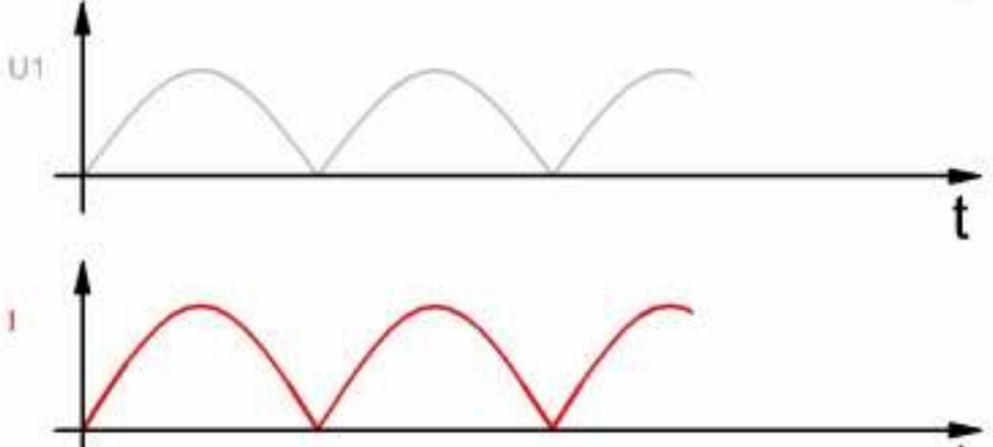
\includegraphics[width=0.9\linewidth]{images/PrakUGB2Kl2}
\end{minipage}
\begin{minipage}{0.35\linewidth}
    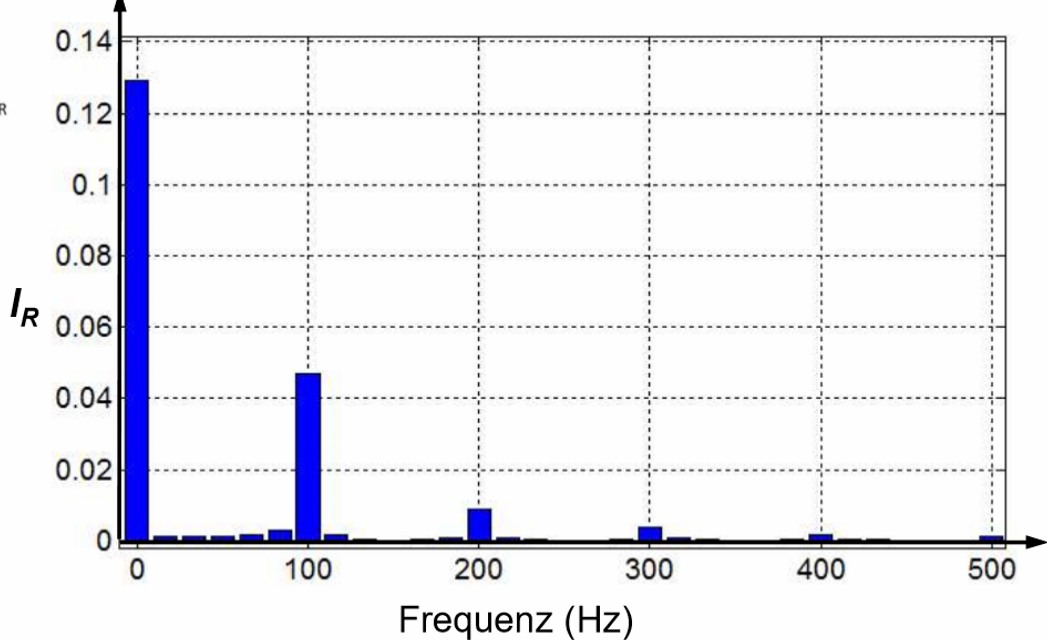
\includegraphics[width=\linewidth]{images/UGB2OW}
\end{minipage}\newline

Im gegensatz zur M1U-Schaltung wird hier die negative Netzspannung zur Gleichrichtung genutzt.\newline
Die Schaltung wird oft mit Glättungskondensator betrieben.
\begin{longtable}{| p{.33\textwidth} | p{.40\textwidth} | p{.25\textwidth} |} %TODO Formeln einfügen
    \hline
    \textbf{Grundgleichungen}&
    \[ \bar{U}_{OUT} = 2\dfrac{\hat{U}}{\pi}\]&\\
    \hline   
\end{longtable}

%===================================================================
%\clearpage

\subsubsection{B6U}
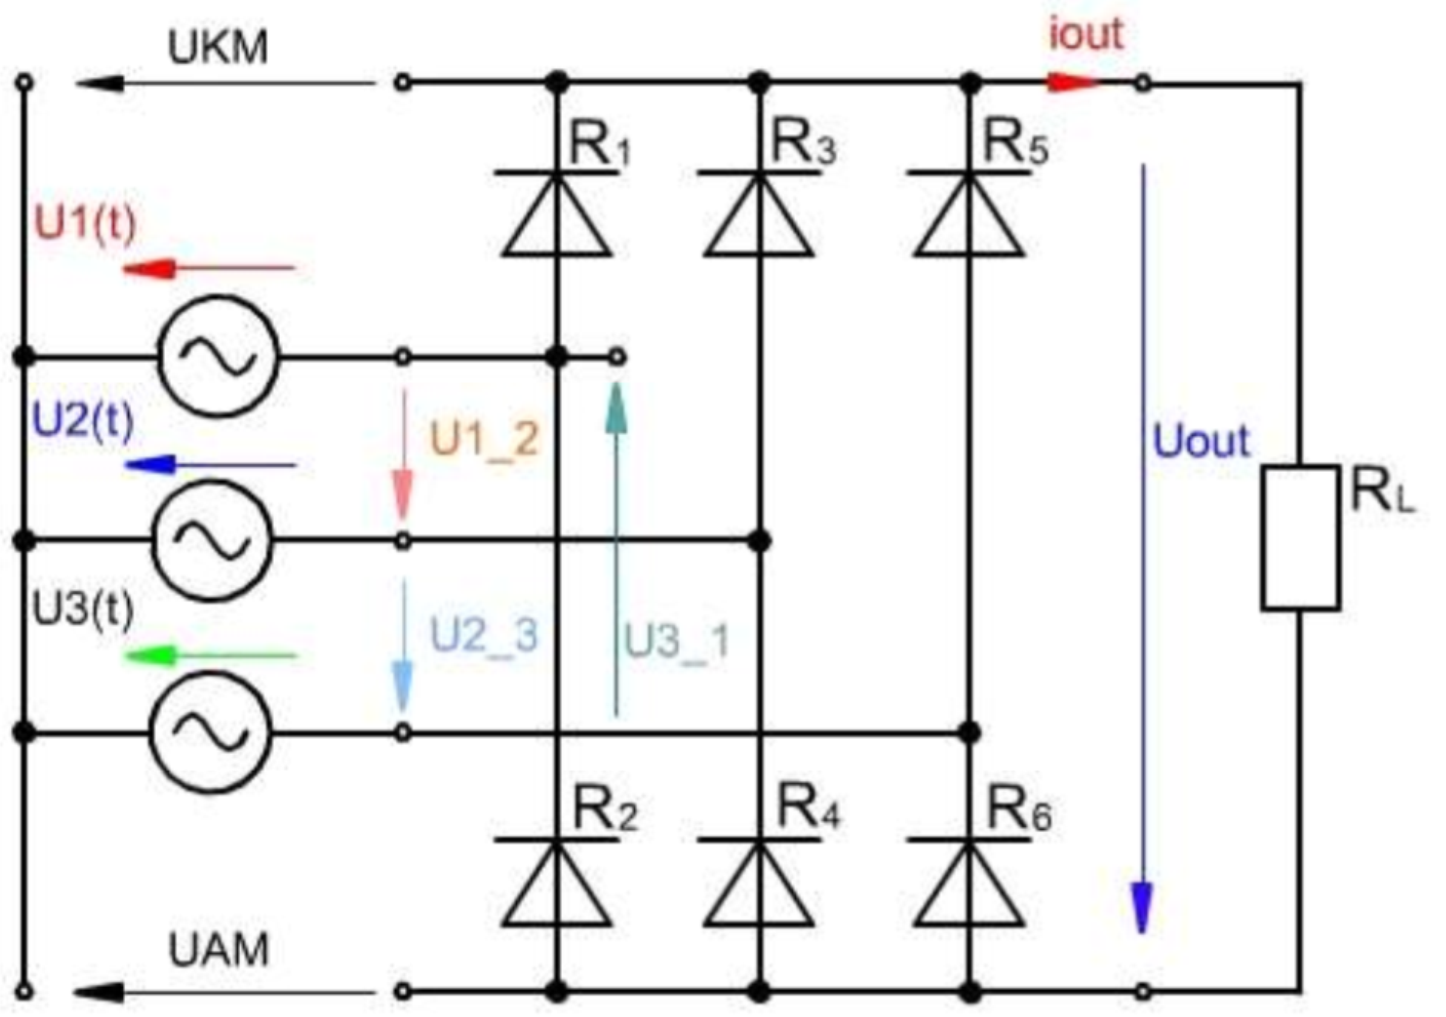
\includegraphics[width=0.3\linewidth]{images/PrakUGB6}
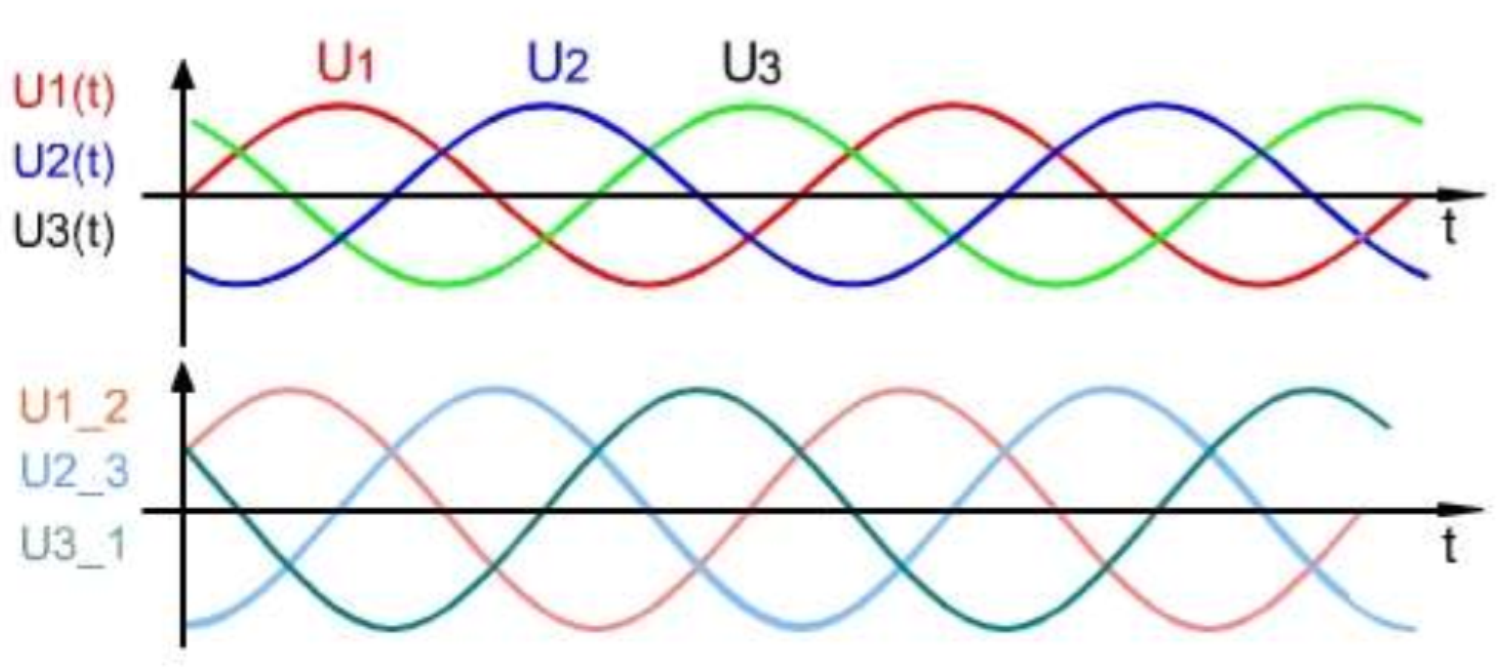
\includegraphics[width=0.3\linewidth]{images/PrakUGB6Kl1}
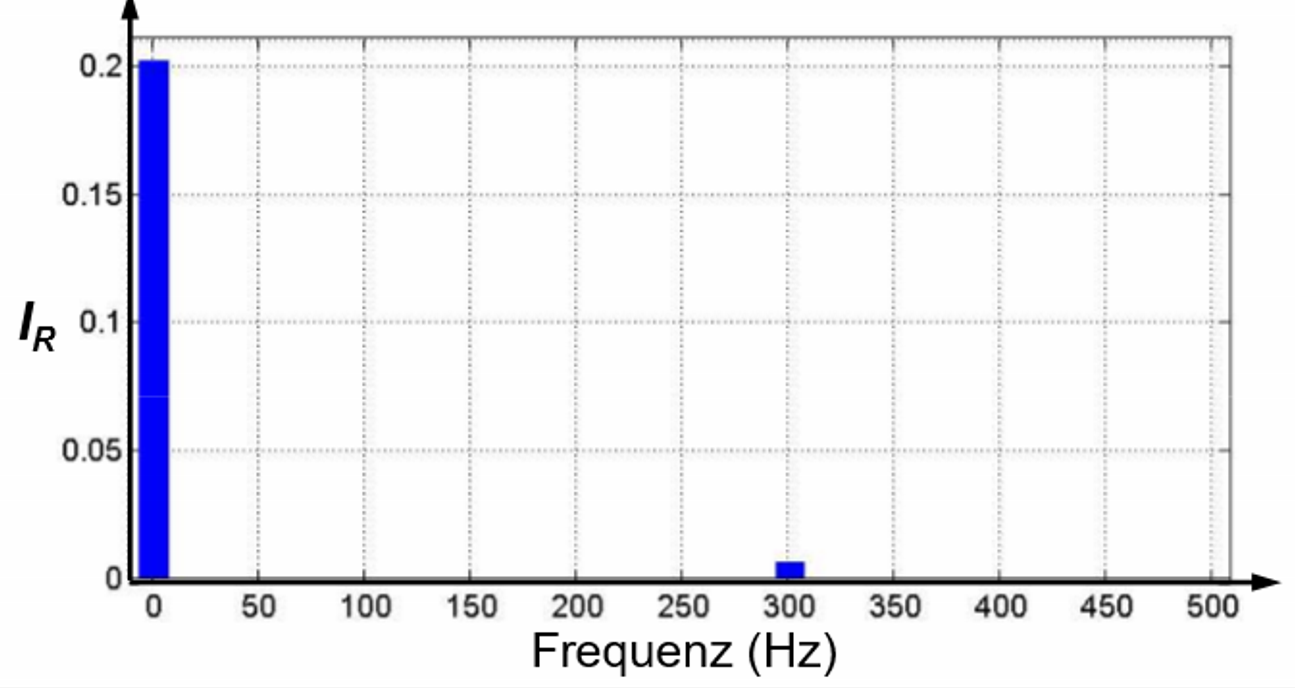
\includegraphics[width=0.3\linewidth]{images/UGB6OW}\newline
\clearpage